\section{List 列表}

\begin{Java}
public interface List<E> extends Collection<E>
\end{Java}

List 接口继承自 Collection 接口,新增了以下方法:

\begin{Java}
// get 与 set 方法
E get(int index);
E set(int index, E element);
// 搜索元素下标
int indexOf(Object o);
int lastIndexOf(Object o);
// 获取子列表
List<E> subList(int fromIndex, int toIndex);
\end{Java}

此外,还提供了一个静态的 of 方法,用于获取不可变的列表。

\begin{Java}
static <E> List<E> of(E... elements)
\end{Java}

AbstractList 是 List 的默认实现。

Java 中有四个主要的 List 容器,他们都直接或简介继承/实现了 List 接口与 AbstractList 抽象类,他们的主要继承关系如下:

\begin{center}
    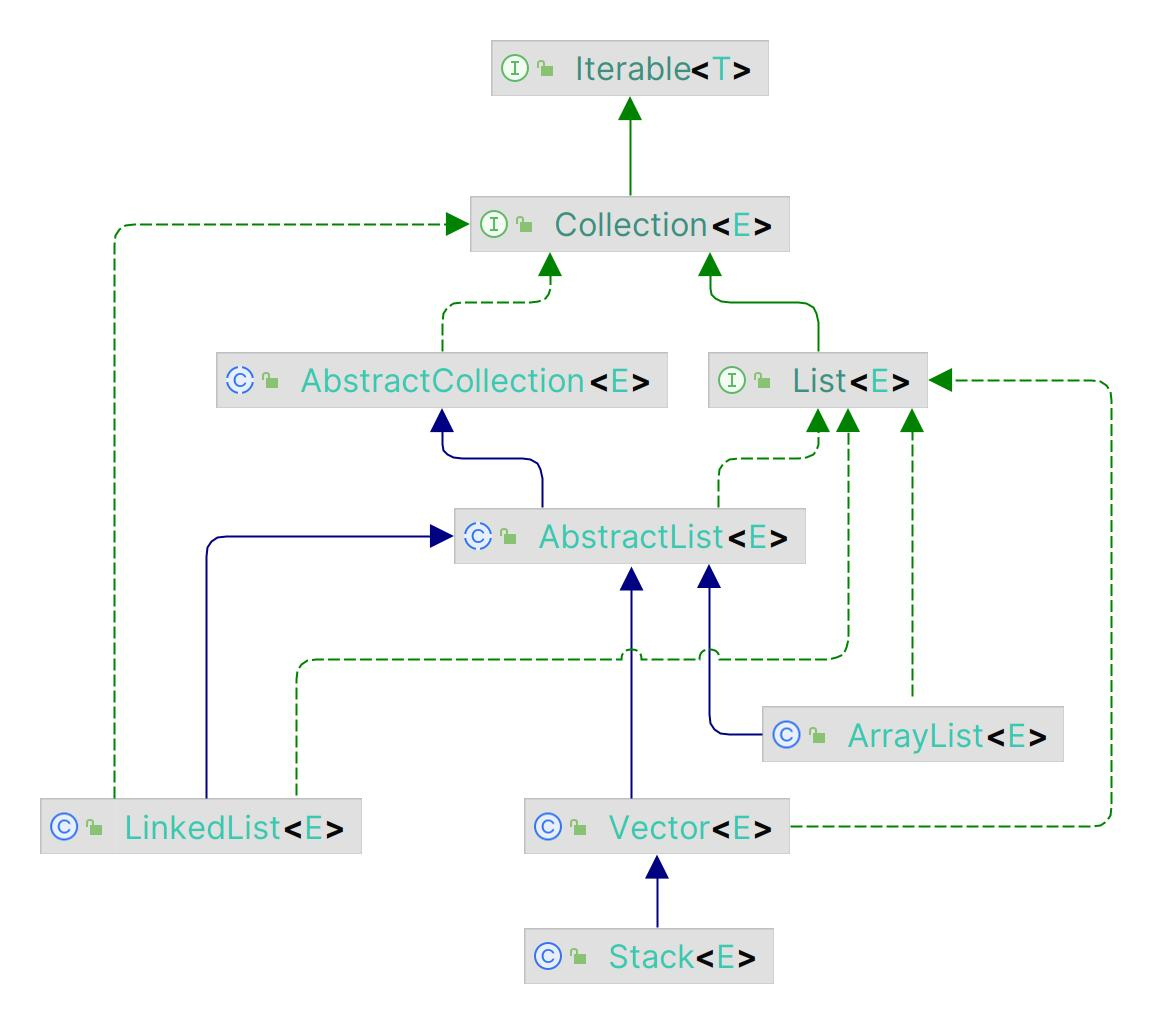
\includegraphics[width=0.6\linewidth]{../../../imgs/List.jpg}
\end{center}

\subsection{ArrayList}

ArrayList 是列表中最常用的容器,底层基于数组实现容器大小动态变化,允许 null 存在。一般的,使用列表这种数据结构无脑选 ArrayList。

\begin{Java}
public class ArrayList<E> extends AbstractList<E> implements List<E>, RandomAccess, Cloneable, java.io.Serializable
\end{Java}

其中 RandomAccess 是一个标记接口,表示可以随机访问,ArrayList 底层是数组,自然可以通过下标快速随机访问。

\subsubsection{数据存储机制}

ArrayList 有一个核心的成员变量 elementData 用于存储数据:

\begin{Java}
transient Object[] elementData;
\end{Java}

这里有个问题,ArrayList 继承了 Serializable 接口,是可以序列化的,但是存储数据的 elementData 被 transient 修饰,说明 elementData 不想被序列化。

这是因为序列化ArrayList的时候,ArrayList里面的elementData未必是满的,比方说elementData有10的大小,但是我只用了其中的3个,就没有必要序列化整个 elementData,具体序列化方式放在了 writeObject 方法中:

\begin{Java}
@java.io.Serial
private void writeObject(java.io.ObjectOutputStream s)
    throws java.io.IOException {
    int expectedModCount = modCount;
    // 序列化非 transient 元素
    s.defaultWriteObject();
    s.writeInt(size);
    for (int i=0; i<size; i++) {
        s.writeObject(elementData[i]);
    }
    if (modCount != expectedModCount) {
        throw new ConcurrentModificationException();
    }
}
\end{Java}

此外,还有几个重要的成员变量:

\begin{Java}
// 记录实际大小,每次增减元素都会改变
private int size;
// 记录被修改的次数
protected transient int modCount = 0;
\end{Java}
 
在 ArrayList 数据更改的过程中,核心操作时调用 Arrays.copyOf 方法对数组进行复制,常见的方法如下:

\begin{Java}
// 构造方法。本质上是根据参数给 elementData 加数据
public ArrayList(int initialCapacity) {
    if (initialCapacity > 0) {
        this.elementData = new Object[initialCapacity];
    } else if (initialCapacity == 0) {
        this.elementData = EMPTY_ELEMENTDATA;
    } else {
        throw new IllegalArgumentException("Illegal Capacity: "+ initialCapacity);
    }
}
// clone 方法
public Object clone() {
    try {
        ArrayList<?> v = (ArrayList<?>) super.clone();
        v.elementData = Arrays.copyOf(elementData, size);
        v.modCount = 0;
        return v;
    } catch (CloneNotSupportedException e) {
        throw new InternalError(e);
    }
}
\end{Java}

transient 还有很多类似的用法,其本质都是通过优化序列化过程减轻数据传输与存储压力,下文不再赘述。

\subsubsection{扩容机制}

\fbox{
    \parbox{0.87\textwidth}{
        \begin{notice}
            本人查资料的时候发现,JDK8 与 JDK17 扩容机制的核心代码有很大不同,本文以 JDK17 为准。
        \end{notice}
    }
}

ArrayList 的强大之处就在于它实现了数组长度的动态变化,本质上还是 Arrays.copyOf 复制数组。理解扩容机制的切入点是 add 方法:

\begin{Java}
public boolean add(E e) {
    modCount++;
    add(e, elementData, size);
    return true;
}

private void add(E e, Object[] elementData, int s) {
    if (s == elementData.length)
        elementData = grow();
    elementData[s] = e;
    size = s + 1;
}
\end{Java}

往下找,可以找到扩容机制的核心方法: grow

\begin{Java}
private Object[] grow() {
    return grow(size + 1);
}

private Object[] grow(int minCapacity) {
    int oldCapacity = elementData.length;
    // 非空列表扩容
    if (oldCapacity > 0 || elementData != DEFAULTCAPACITY_EMPTY_ELEMENTDATA) {
        // newCapacity 是旧容器的 1.5 倍
        int newCapacity = ArraysSupport.newLength(oldCapacity,
                minCapacity - oldCapacity, /* minimum growth */
                oldCapacity >> 1           /* preferred growth */);
        return elementData = Arrays.copyOf(elementData, newCapacity);
    // 空列表扩容
    } else {
        // 10 或 要扩的大小
        return elementData = new Object[Math.max(DEFAULT_CAPACITY, minCapacity)];
    }
}
\end{Java}

因此,我们可以进行总结: 如果是一个空列表,扩容增加 10,如果不是,扩容增加 1.5 倍。这里有两个注意点:

\begin{itemize}
    \item 对于空列表,ArrayList 有一个 static final 的空数组,每次都会调用它,是个小优化。
    \item 对于 1.5 倍扩容,采用的是去尾法,15 $\rightarrow$ 22,但是 1 会扩为 2。
\end{itemize}

此外,ArrayList 还提供了一个缩容方法:

\begin{Java}
public void trimToSize() {
    modCount++;
    if (size < elementData.length) {
        elementData = (size == 0)
          ? EMPTY_ELEMENTDATA
          : Arrays.copyOf(elementData, size);
    }
}
\end{Java}

可以手动调用该方法对容器进行缩容。

\subsection{LinkedList}

LinkedList 使用双向链表实现列表。理论上 ArrayList 更适合查询,LinkedList 更适合插入操作.但实际运用中,除非是头部或者尾部插入,LinkedList 会有明显的优势(因为要先查询再插入),其他方面并没有任何优势,并且 LinkedList 需要维护链表指针有一定的空间开销,所以在要使用列表结构时 LinkedList 很少用。

因为 LinkedList 比较少用,所以这里不做过多讲解。

\begin{Java}
public class LinkedList<E> extends AbstractSequentialList<E> implements List<E>, Deque<E>, Cloneable, java.io.Serializable
\end{Java}

这里可以看到 LinkedList 直接继承自 AbstractSequentialList, AbstractSequentialList 又直接继承自 AbstractList。AbstractSequentialList 提供了一套基于顺序访问的接口。它提供的方法基本上都是通过 ListIterator 实现。

\subsubsection{Node 节点}

既然是链表结构,拿必然有节点元素,LinkedList 内部有两个只想头部和尾部的节点。

\begin{Java}
transient Node<E> first;
transient Node<E> last;
\end{Java}

发现又是 transient 修饰的,查看序列方法:

\begin{Java}
@java.io.Serial
private void writeObject(java.io.ObjectOutputStream s)
    throws java.io.IOException {
    s.defaultWriteObject();
    s.writeInt(size);
    for (Node<E> x = first; x != null; x = x.next)
        s.writeObject(x.item);
}
\end{Java}

发现传的时候只会依次穿节点中的数据, 节点本身被抛弃了。

Node 本身是 LinkedList 的一个内部类:

\begin{Java}
private static class Node<E> {
    E item;
    Node<E> next;
    Node<E> prev;
    Node(Node<E> prev, E element, Node<E> next) {
        this.item = element;
        this.next = next;
        this.prev = prev;
    }
}
\end{Java}

常用的方法没什么好介绍的,无非是一些常规的链表操作,看一下构造函数和常用方法:

\begin{Java}
public LinkedList() { }
public LinkedList(Collection<? extends E> c) {
    this();
    addAll(c);
}
\end{Java}

其中 addAll 并没有调用 add 方法,而是迭代插入新节点。原因之一是这样 modCount 只会加一。

此外,clear 操作也进行了优化,将每个节点的引用关系都赋空,主要是方便 GC:

\begin{Java}
public void clear() {
    for (Node<E> x = first; x != null; ) {
        Node<E> next = x.next;
        x.item = null;
        x.next = null;
        x.prev = null;
        x = next;
    }
    first = last = null;
    size = 0;
    modCount++;
}
\end{Java}

LinkedList 还实现了很多队列操作,这里不做说明。

\subsection{Vector}

Vector 是 List 的古早实现,现在已经被 ArrayList 代替,但是 Vector 是线程安全的,ArrayList 和 LinkedList 是线程不安全的。当然,可以从 Collections 调用 synchronizedList 方法获取线程安全列表。

\begin{Java}
public class Vector<E> extends AbstractList<E> implements List<E>, RandomAccess, Cloneable, java.io.Serializable
\end{Java}

Vector 的主要成员方法如下:
\begin{Java}
protected Object[] elementData;
protected int elementCount;
protected int capacityIncrement;
\end{Java}

和 ArrayList 不同,没有对 elementData 添加 transient 关键字。

另外不同的是,Vector 需要在构造时指定扩容大小:

\begin{Java}
public Vector(int initialCapacity, int capacityIncrement)
\end{Java}

它的扩容机制核心代码如下:

\begin{Java}
private Object[] grow(int minCapacity) {
    int oldCapacity = elementData.length;
    int newCapacity = ArraysSupport.newLength(oldCapacity,
            minCapacity - oldCapacity, /* minimum growth */
            capacityIncrement > 0 ? capacityIncrement : oldCapacity
                                       /* preferred growth */);
    return elementData = Arrays.copyOf(elementData, newCapacity);
}
\end{Java}

这里只有一句和 ArrayList 不同: capacityIncrement > 0 ? capacityIncrement : oldCapacity
\begin{itemize}
    \item 如果没有显示指定 capacityIncrement 大小,capacityIncrement 为0,因此每次扩容大小为初始 Vector 大小。
    \item 如果显示制定了 capacityIncrement 大小,每次按 capacityIncrement 大小扩容。
\end{itemize}

此外,Vector 线程安全的原理是加了 synchronized 关键字。具体方法实现和 ArrayList 差别不大。

\subsection{Stack}

从数据结构上讲,栈应该是独立于列表的一种数据结构,Java 中 Stack 继承自 Vector,因此 Stack 保留了许多和 ArrayList,Vector 类似的性质,且是线程安全的。

\begin{Java}
public class Stack<E> extends Vector<E>
\end{Java}

它新增的方法如下:

\begin{Java}
// 无参构造函数,就这一个构造函数
public Stack()
// 压栈,就调用了一个 synchronized 方法,所以无需 synchronized 关键字
public E push(E item)
// 弹栈
public synchronized E pop()
// 看栈顶元素
public synchronized E peek()
// 判空: 和 push 类似,线程安全
public boolean empty()
    return size() == 0;
// 查找,返回的是与栈顶的距离
public synchronized int search(Object o)
\end{Java}

\newpage